\section{Искуственные нейронные сети}

\indent
\indent
Настоящая часть работы предназначена для читателя, не знакомого с 
искуственными нейронными сетями и глубоким обучением. 
Здесь будут приведены теоретические 
основы глубокого обучения и рассмотрены сверточные архитектуры, 
используемые в дальнейшей работе.


\subsection{Перцептрон}

\indent
Начнем с рассмотрения одиночного нейрона
 --- перцептрона Розенблатта --- базового элемента, содержащегося в большинстве современных нейросетевых архитектур.
Перцептрон имеет несколько входов и один выход, значение на котором
вычисляется как взвешенная сумма значений входов 
(рисунок \ref{tikzpicture: perceptron}).
Кроме того, обычно
к выходному значению применяется сдвиг и некоторая нелинейная функция, 
называющаяся функцией активации нейрона. Ее предназначение мы обсудим позже.

\begin{figure}[h!]
    \begin{center}
   	    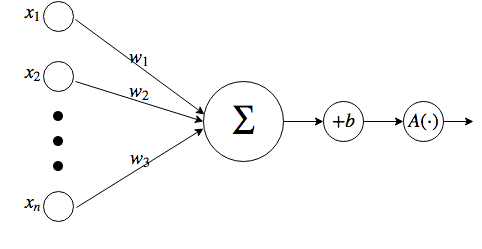
\includegraphics[width=0.6\linewidth]{Perceptron}
   	\end{center}
   	\caption{Схематическое изображение работы одного отдельного нейрона.}
   	\label{tikzpicture: perceptron}
\end{figure}


\indent
\indent
Таким образом, значение на выходе нейрона задается
 выражением \ref{eq:perceptron}.

\begin{equation}\label{eq:perceptron}
    f(\vec{x}) = S(\sum_{i=1}^n x_i w_i + b)
\end{equation}


где $f(\vec{x})$ -- выходное значение нейрона, посчитанное для входов $x_i$,
$w_i$ -- весовые коэффициенты для каждого входа, $b$ -- параметр смещения, 
а $S$ --- нелинейная функция активации. Далее для упрощения повествования
положим $b \equiv 0$.

\subsection{Функции активации}

\indent
\indent
Существуют множество различных функций активации, например, гиперболический
тангенс, логистическая сигмоида или \textit{ReLU}, рисунок \ref{tikzpicture: activations}.

\begin{equation}\label{eq:activations}
	\begin{gathered}
	    S(x) = th(x) = \frac{e^x - e^{-x}}{e^x + e^{-x}},    \;   th’(x) = {1 - th(x)^2}  \\    
	    S(x) = \sigma(x) = \frac{1}{1 + e^{-2x}},   \;   \sigma’(x) = \sigma(x)(1 - \sigma(x)) \\
	    S(x) = ReLU = max(0, x),   \;   ReLU’(x) = \theta(x)
	\end{gathered}
\end{equation}
где $\theta(x)$ -- функция Хэвисайда.

\indent
\indent
Эти функции используются
для добвления нелинейных зависимостей между слоями многослойной модели.
Названные выше функции особенно популярны, 
так как значения их производных либо достаточно просты, либо легко 
выражаются через значения самих функций (выражение \ref{eq:activations}), 
что позволяет быстро вычислять значение производной.

\begin{figure}[h!]
	\begin{center}
		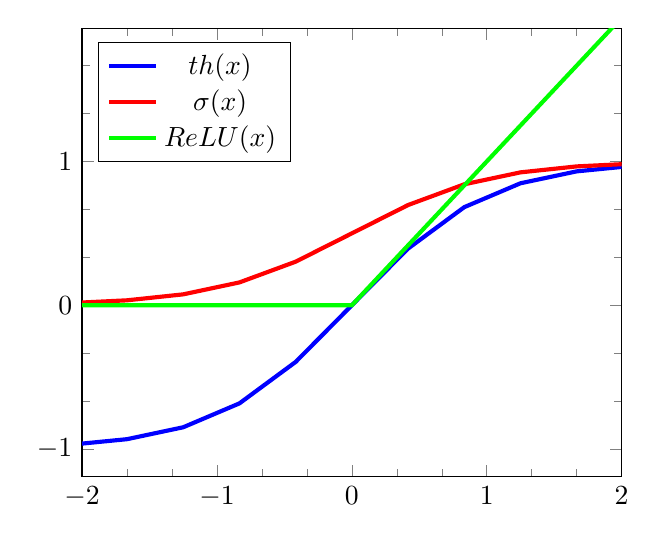
\begin{tikzpicture}
			\begin{axis} [
			    legend pos = north west, 
			    xmin = -2,
			    xmax = 2,
			    minor tick num = 2
			]
			\legend{ 
				$th(x)$, 
				$\sigma(x)$, 
				$ReLU(x)$
			};
			\addplot[blue, line width = 1.5] {tanh(x)};
			\addplot[red, line width = 1.5] {1 / (1 + e^(-2*x))};
			\addplot[green, line width = 1.5] {max(0, x)};
			\end{axis}
		\end{tikzpicture}
	\end{center}
\caption{Функции активации}
\label{tikzpicture: activations}
\end{figure}

\subsection{Полносвязная сеть}

\indent
\indent
Одиночный нейрон не способен выразить сложные в наборе
признаков $\vec{x}$, поэтому нейроны объединяют в слои, а их, в свою 
очередь, в многослойные сети . Рассмотрим сеть,
состоящую из двух слоев нейронов. Пусть количество количество входных признаков
равно $N$, количество нейронов скрытого слоя $P$,
а размер выхода -- $M$, рисунок \ref{tikzpicture: fc_net}. Такая архитектура, 
состоящая из простых линейных слоев, называется полносвязной.
 
\begin{figure}[h!]
    \begin{center}
   	    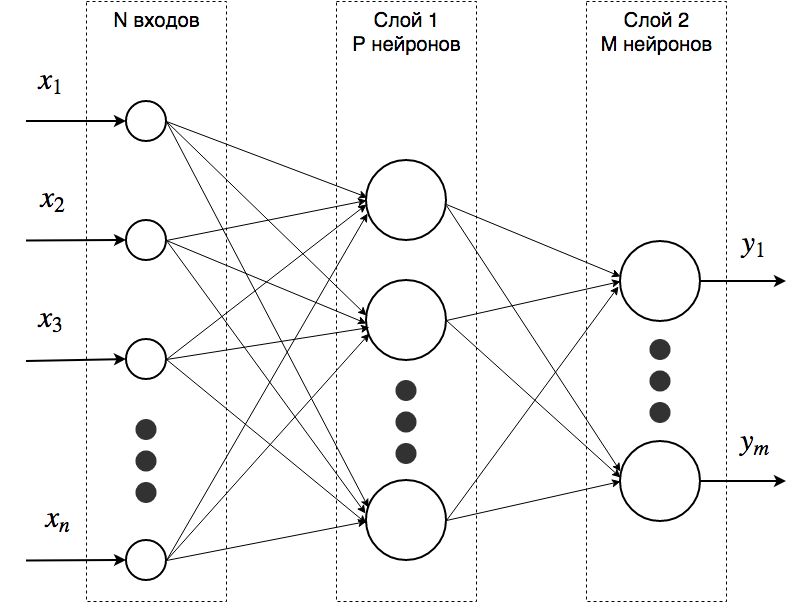
\includegraphics[width=0.9\linewidth]{FC_net}
   	\end{center}
   	\caption{Схематическое изображение полносвязной нейронной сети.}
   	\label{tikzpicture: fc_net}
\end{figure}

Рассмотрев выражение \ref{eq:perceptron} можно увидеть, что 
совокупность значений нейронов на 1 слое может быть получена 
простым матричным умножением входов $\vec{x}$ на матрицу весов
 $W^1$ размера $P \times N$, с последующим поэлементным применением 
функции активации к получившися значениям. Аналогично, значения нейронов
2 слоя получаются умножением предыдущих значений на весовую матрицу
$W^2$ размером $M \times P$. Таким образом, применение нейросети
ко входу $\vec{x}$ можно задать выражением \ref{eq:forward}.

\begin{equation}\label{eq:forward}
	   \vec{y} = W^{2} S(W^{1} \vec{x})
\end{equation}
где $S(\cdot)$ -- применение нелинейности к каждому элементу входного 
вектора.

\subsection{Функция потерь}

\indent
\indent
Близость предсказания сети к правильным ответам оценивается
с помощью функции ошибки, так же называемой 
 функцией потерь \textit{(loss function)}. 
Например, для задачи регресии в качестве функции потерь
может применяться среднеквадратичное отклонение
 (\textit{MSE}, выражение \ref{eq: mse}),
 или, в более простом случае -- средняя разность между выходами модели и правильными ответами (выражение \ref{eq:diff});
для задачи классификации обычно используют перекрестную энтропию 
(\textit{cross entropy}, выражение \ref{eq: cross_entropy}).


\begin{equation}\label{eq:diff}
        L_{1}(\vec{y_{gt}}, \vec{y}) = \frac{1}{M} \sum_{i=1}^M | y^{gt}_{i} - y_{i} |
\end{equation}

\begin{equation}\label{eq: mse}
    MSE(\vec{y_{gt}}, \vec{y}) = \frac{1}{M} \sum_{i=1}^M (y^{gt}_{i} - y_{i})^2
\end{equation}

\begin{equation}\label{eq: cross_entropy}
    CE(\vec{y_{gt}}, \vec{y}) = - \sum_{i=1}^M y_{i} \log{y^{gt}_{i}}
\end{equation}

\indent
\indent
Исходя из постановки решаемой задачи, можно составить и другие функции ошибок, но
они обязательно должны быть дифференциируемыми.
Это необходимо условие, чтобы использовать метод обратного распространения
ошибки для обучения модели.


\subsection{Метод обратного распространения ошибки}
% https://habr.com/ru/company/ods/blog/344116/
% https://ru.wikipedia.org/wiki/Метод_обратного_распространения_ошибки

\indent
\indent
Поняв, как конструируются нейронные сети, что представляют собой функции активации
и функции потерь, обсудим, как происходит обучение моделей.

\subsection{Сверточные нейронные сети}
\indent
\indent
Сверточная неройнная сеть \textit{(Convolution neural network)} --- 
это специальная сеть, сконструированная для 
обработки изображений, хотя в настоящее время спектр их применения 
значительно расширился. Как следует из названия, основной таких сетей 
являются сверточные слои \textit{convolutional layers}.
Кроме того, обычно вместе с ними используются такие
слои как \textit{BatchNormalization}, \textit{Pooling}, \textit{Softmax} и \textit{Dropout}.

\indent
\indent
Рассмотрим, как устроено применение оператора свертки к изображению.
% https://habr.com/ru/company/ods/blog/344008/

\subsection{Используемые сверточные архитектуры}
\indent
\indent
В данное работе используются следующие архитектуры нейронных сетей:


\begin{itemize}

    \item \textit{Residual netwrotk (ResNet)} ---
    одна из самых популярных в настоящее время архитектур,
    предложенная в статье \cite{resnet} 2015 года.
    Основная идея состоит в добавлении конкатенации значений
    нейронов на \textit{i-м} слое с \textit{i-2} слоем (такая процедура
    получила название \textit{skip connection}. Таким образом авторы
    успешно решают распространенную проблему обучения глубоких сетей ---
    затухание градиентов.
    
    \item {Inception} --- todo
    
    \item {DenseNet} --- todo
    
    \item {VGG} --- относительно старая, ставшая классической, архитектура,
    предложенная в 20хх году todo.
    
\end{itemize}

